\documentclass[10pt]{article}
%\usepackage[UTF8]{ctex}

\usepackage[utf8]{inputenc} % allow utf-8 input

\usepackage{amsmath,amscd}
\usepackage{amssymb,array}
\usepackage{amsfonts,latexsym}
\usepackage{graphicx,subfig,wrapfig}
\usepackage{times}
\usepackage{psfrag,epsfig}
\usepackage{verbatim}
\usepackage{tabularx}
\usepackage[pagebackref=true,breaklinks=true,letterpaper=true,colorlinks,bookmarks=false]{hyperref}
\usepackage{cite}
\usepackage{algorithm}
\usepackage{multirow}
\usepackage{caption}
\usepackage{algorithmic}
\usepackage[amsmath,thmmarks]{ntheorem}
\usepackage{listings}
\usepackage{color}

\usepackage{enumitem}
\usepackage[most]{tcolorbox}
\tcbuselibrary{breakable}
\newtcolorbox{mybox}{
	breakable,
    arc=0pt,
    boxrule=1pt,
    % colback=red,
    % width=.8\textwidth,   % this option controls the width of the box
    colupper=blue,
    % fontupper=\bfseries
}


\newtheorem{thm}{Theorem}
\newtheorem{mydef}{Definition}

\DeclareMathOperator*{\rank}{rank}
\DeclareMathOperator*{\trace}{trace}
\DeclareMathOperator*{\acos}{acos}
\DeclareMathOperator*{\argmax}{argmax}


\renewcommand{\algorithmicrequire}{ \textbf{Input:}}     
\renewcommand{\algorithmicensure}{ \textbf{Output:}}
\renewcommand{\mathbf}{\boldsymbol}
\newcommand{\mb}{\mathbf}
\newcommand{\matlab}[1]{\texttt{#1}}
\newcommand{\setname}[1]{\textsl{#1}}
\newcommand{\Ce}{\mathbb{C}}
\newcommand{\Ee}{\mathbb{E}}
\newcommand{\Ne}{\mathbb{N}}
\newcommand{\Se}{\mathbb{S}}
\newcommand{\norm}[2]{\left\| #1 \right\|_{#2}}

\newenvironment{mfunction}[1]{
	\noindent
	\tabularx{\linewidth}{>{\ttfamily}rX}
	\hline
	\multicolumn{2}{l}{\textbf{Function \matlab{#1}}}\\
	\hline
}{\\\endtabularx}

\newcommand{\parameters}{\multicolumn{2}{l}{\textbf{Parameters}}\\}

\newcommand{\fdescription}[1]{\multicolumn{2}{p{0.96\linewidth}}{
		
		\textbf{Description}
		
		#1}\\\hline}

\newcommand{\retvalues}{\multicolumn{2}{l}{\textbf{Returned values}}\\}
\def\0{\boldsymbol{0}}
\def\b{\boldsymbol{b}}
\def\bmu{\boldsymbol{\mu}}
\def\e{\boldsymbol{e}}
\def\u{\boldsymbol{u}}
\def\x{\boldsymbol{x}}
\def\v{\boldsymbol{v}}
\def\w{\boldsymbol{w}}
\def\N{\boldsymbol{N}}
\def\X{\boldsymbol{X}}
\def\Y{\boldsymbol{Y}}
\def\A{\boldsymbol{A}}
\def\B{\boldsymbol{B}}
\def\y{\boldsymbol{y}}
\def\cX{\mathcal{X}}
\def\transpose{\top} % Vector and Matrix Transpose

%\long\def\answer#1{{\bf ANSWER:} #1}
\long\def\answer#1{}
\newcommand{\myhat}{\widehat}
\long\def\comment#1{}
\newcommand{\eg}{{e.g.,~}}
\newcommand{\ea}{{et al.~}}
\newcommand{\ie}{{i.e.,~}}

\newcommand{\db}{{\boldsymbol{d}}}
\renewcommand{\Re}{{\mathbb{R}}}
\newcommand{\Pe}{{\mathbb{P}}}

\hyphenation{MATLAB}

\usepackage[margin=1in]{geometry}

\begin{document}
	
\title{Machine Learning, 2021 Spring\\Homework 4}
\date{Due on 23:59 MAY 5, 2021
	}
\maketitle

%%%%%--------------------

% \section*{Problem 1}
% Please refer to {\color{red}slides p7-11 in Lecture 9: Feasibility of Learning}. The definition of the following symbol is the same as that in lecture.
% \begin{enumerate}
% \item Using binomial distribution, find the probability that a sample of 10 marbles will have $v \leq 0.1$ given that $\mu = 0.9$. (15 points)
% \item Using Hoeffding Inequality to bound the probability that a sample of 10 marbles will have $v \leq 0.1$ given that $\mu = 0.9$. (15 points)
% \end{enumerate}

% \begin{mybox}
% Maybe this problem has been released in HW1.
% \end{mybox}

\textbf{Please submit your homework in ``pdf'' format. Submit the supplementary materials (e.g., files for code) in an {\color{red}extra} ``zip'' file.}

\section*{Problem 1} 
For a random variable $z$, let $\bar z$ denote its mean, \emph{i.e.}, $\bar{z}=\mathbb{E}[z]$. 

Suppose we are given a dataset $\mathcal{D}=\{x^{(i)},y^{(i)}\}_{i=1}^m$ drawn \emph{i.i.d.} from some \emph{unknown} distribution $P(X,Y)$. Given $x$, the expected label is defined as
\begin{equation}
    \bar{y}(x) = \mathbb{E}_{y|x}[Y]
\end{equation}
which denotes the label we would expect to obtain.

Next, we run some learning algorithm, such as SVM, linear regression, from which we learned our hypothesis function $h_{\mathcal{D}}$. 

Now for a new data point $(x,y)$ sampled from $P(X,Y)$ and out of $\mathcal{D}$, we want to investigate the expected error between the predicted value $h_{\mathcal{D}}(x)$ and the observation $y$, \emph{i.e.},
\begin{equation}
\mathbb{E}_{\mathcal{D},x,y}[(y-h_{\mathcal{D}}(x))^2].
\end{equation}

This error can be decomposed into three parts namely: \textbf{variance}, $\textbf{bias}$, and \textbf{noise}, where the expectation is taken over all possible training set $\mathcal{D}$ and all $(x,y)$. Here
\begin{equation}
\begin{aligned} 
\textbf{bias}^2 &=\ \mathbb{E}_{x}[(\bar{y}(x)-\bar{h}(x))^2]\\
\textbf{variance} &=\ \mathbb{E}_{x,\mathcal{D}} [(\bar{h}(x)-h_{\mathcal{D}}(x))^2]\\
\textbf{noise} &=\ \mathbb{E}_{x,y}[(y-\bar{y}(x))^2]
\end{aligned}
\end{equation}
where $\bar{h}(x)=\mathbb{E}_{\mathcal{D}}[h_{\mathcal{D}}(x)]$ is the ``average approximator'' by averaging classifiers on all possible training dataset $\mathcal{D}$.

 
The error \textbf{bias} is the amount by which the expected model prediction differs from the true value or target; while \textbf{variance} measures how inconsistent are the predictions from one another, over different training sets, not whether they are accurate or not. \textbf{Models that exhibit small variance and high bias underfit the truth target. Models that exhibit high variance and low bias overfit the truth target}.

The data scientist’s goal is to simultaneously reduce bias and variance as much as possible in order to obtain as accurate model as is feasible. However, there is a trade-off to be made when selecting models of different flexibility or complexity and in selecting appropriate training sets to minimize these sources of error.

\textbf{Question}:  {\color{red} [2 pts]}

Show that
\begin{equation}
    \mathbb{E}_{\mathcal{D},x,y}[(y-h(x))^2] = \textbf{variance}+\textbf{bias}^2+\textbf{noise}.
\end{equation}


% Hints: first you may want to prove a lemma that for any random variable, it holds true that
% $$
% \mathbb{E}[(z-\bar z)^2] = \mathbb{E}[z^2]-\bar{z}^2,
% $$
% so that
% $$
% \mathbb{E}[z^2]=\mathbb{E}[(z-\bar z)^2+\bar{z}^2].
% $$
% It follows that $(y-h(x))^2 = y^2 - 2h(x)y+h(x)^2$. Note that $y$ and $h(x)$ are independent variables. The result follows from using the lemma twice. Also note $\mathbb{E}_{x,y}[(y-f(x))^2]=\sigma^2$.  (20 points)









\section*{Problem 2}
Given the training dataset ``data/crime-train.txt"  and the test dataset ``data/crime-test.txt'' (For more information about the datasets, you may refer to ``README.md").

We'd like to use the training dataset to fit a model which can predict the crime rate in new communities, and evaluate model performance on the test set. As there are a considerable number of input variables, overfitting is a serious issue. In order to avoid this, we will use the L2 regularization. 

The main goal of this homework is to give you some experience using L2 regularization as a method for variable selection and using 10-folder cross-validation as a technique to get an insight on how the model will generalize to an independent dataset.
Your function should accept a scalar value of $\lambda$, a vector-valued response variable ($\mathbf{y}$), a matrix of input variables ($\mathbf{X}$), and an initial vector of weights ($\mathbf{w}_0$). It should output a vector of coefficient values ($\hat{\mathbf{w}}$).

In your analysis, include:
\begin{enumerate}


\item  A plot of $\log(\lambda)$ against the squared error in the 10-folder splited training data. {\color{red} [1 pts]}
\item  A plot of $\log(\lambda)$ against the squared error in the test data. {\color{red} [0.5 pts]}
\item  A plot of $\lambda$ against the number of small coefficients (you can set a threshold), and a brief commentary on the task of selecting $\lambda$. {\color{red} [1 pts]}
\item  For the $\lambda$ that gave the best test set performance, which variable had the largest (most positive) coefficient? What about the most negative? Discuss briefly.  {\color{red} [0.5 pts]}
\end{enumerate}



\section*{Problem 3}
The goal in the prediction problem is to be able to make prediction for the target variable $t$ given some new value of the input variable $x$ on the basis of a set of training data comprising $N$ input values $\mathbf{x} = (x_1,\dots,x_N)^T$ and their corresponding target variable $\mathbf{t}= (t_1,\dots,t_N)^T$. 

We assume that, given the value of $x$ , the corresponding value of $t$ has a Gaussian distribution with a mean equal to the value $y(x,w)$ and the variance $\sigma$, where $y(x,w)$ is the prediction function. For example, for the linear regression, the $y(x,\mathbf{w}) = w_0+w_1x$.

Thus, we have 
\begin{equation}
    p(t|x,\mathbf{w}, \sigma) = \mathcal{N}(t|y(x,\mathbf{w}),\sigma)
\end{equation}
Here we only consider the case of a single real-valued variable $x$.
Now  you need  to use the training data $\{\mathbf{x},\mathbf{t}\}$ to determine the parameter $\mathbf{w}$ and $\sigma$ by maximum likelihood. 
\begin{enumerate}
	\item Show that maximizing the log likelihood is equal to minimizing the sum-of-squares error function. {\color{red} [1 pts]}
	\item More, if we assume that the polynomial coefficients $\mathbf{w}$ is distributed as the Gaussian distribution of the form
	\begin{equation}
	    p(\mathbf{w}|\alpha) =  \mathcal{N}(\mathbf{w}|\mathbf{0},\alpha \mathbf{I})
	\end{equation}
	where $\alpha$ is the parameter of the distribution.
	Then what is the formulation of the prediction problem?  And give us the regularization parameter. Please show us the induction of the procedure.\\
	(Hint. Using Bayes' theorem) {\color{red} [1.5 pts]}
\end{enumerate}


\section*{Problem 4}
In the following problems, we explore the the relationship between the size of the validation set and the expected error. 

Let us first look at how the validation set is created. The first step is
to partition the data set $\mathcal{D}$ of fixed size $N$ into a training set $\mathcal{D}_{train}$ of size $(N-K)$ and a validation set $\mathcal{D}_{val}$ of size $K$. We select $N-K$ points at random for training and the remaining for validation. Figure \ref{fig:problem0} depicts the relationship among $\mathcal{D}$, $\mathcal{D}_{train}$ and $\mathcal{D}_{val}$.
Suppose we have $M$ models $\mathcal{H}_1,\dots,\mathcal{H}_M$. Given $m\in\{1,\dots,M\}$, denote a  $g_m\in\mathcal{H}_m$ as the hypothesis chosen based on data set $\mathcal{D}$,  $g_m^-\in\mathcal{H}_m$ as the hypothesis chosen based on data set $\mathcal{D}_{train}$ as shown in Figure \ref{Fig:modelselection2}.

\begin{figure}[!htb]
   \begin{minipage}{0.48\textwidth}
     \centering
     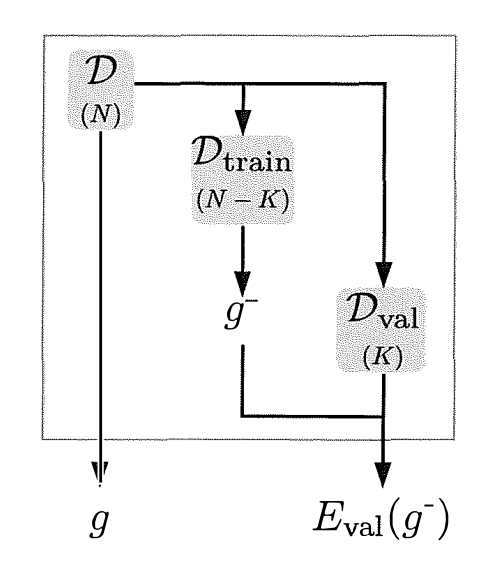
\includegraphics[width=.7\linewidth]{figure/fig0.png}
     \caption{Using a validation set to estimate $E_{out}$}
     \label{fig:problem0}
   \end{minipage}\hfill
   \begin{minipage}{0.48\textwidth}
     \centering
     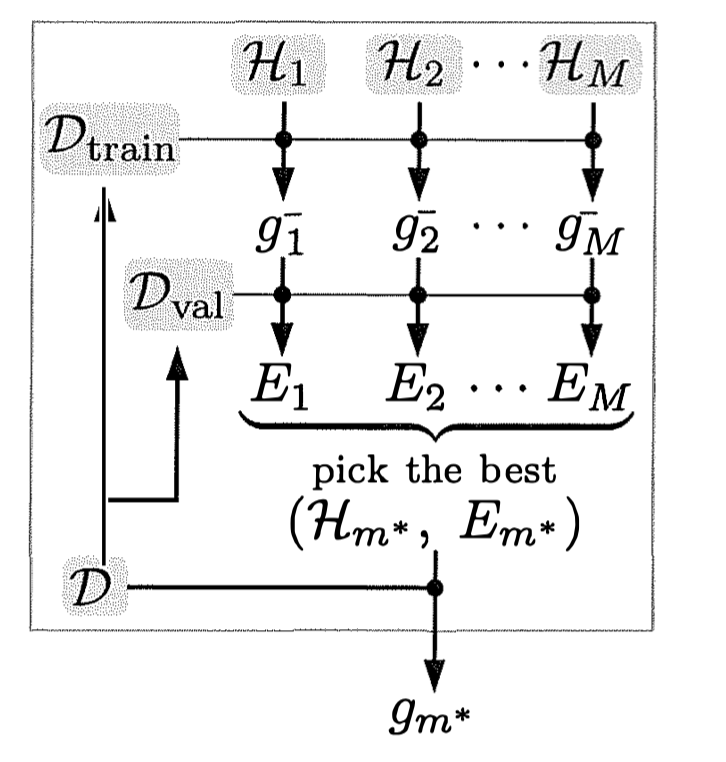
\includegraphics[width=.8\linewidth]{figure/modelSelection.png}
     \caption{Using a validation set for model selection}
     \label{Fig:modelselection2}
   \end{minipage}
\end{figure}

Now we can evaluate each model on the validation set to obtain the validation errors $E_1,\dots,E_M$, where
\begin{equation}
    E_m=E_{val}(g_m^-), \quad m=1,\dots,M
\end{equation}
The validation error can be used as an estimation of the out-of-sample error $E_{out}(g_m^-)$ for each $\mathcal{H}_m$.
It is now a simple matter to select the model with lowest validation error. Let $m^*$ be the index of the model which achieves the minimum validation error. So for $\mathcal{H}_{m^*}$, $E_{m^*}\leq E_{m}$ for $m=1,\dots,M$.

Please answer the following questions:
\begin{figure}[h]
    \centering
    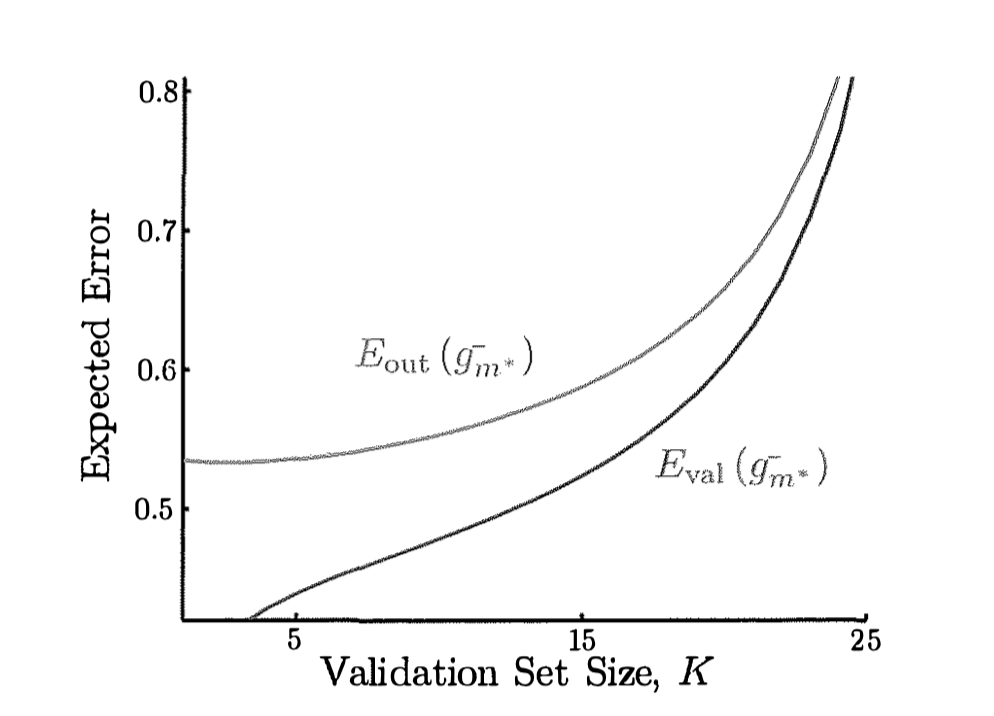
\includegraphics[width=0.7\textwidth]{figure/ExpectedErrorVsValidationSize.png}
    \caption{The out-of-sample error $E_{out}(g_{m^*}^-)$ and the validation error $E_{val}(g_{m^*}^-)$ versus the size $K$ of $\mathcal{D}_{val}$.}
    \label{fig:problem5fig}
\end{figure}
\subsection*{Problem 4a}
Referring to the Figure \ref{fig:problem5fig}, why are both curves increasing with $K$? Why do they converge to each other with increasing $K$? {\color{red} [1 pts]}


\subsection*{Problem 4b}
Referring to the Figure \ref{fig:problem6fig}, answer the following 3 problems:
\begin{enumerate}
	\item $\mathbb{E}\left[E_{out}(g_{m^*}^-)\right]$ is initially decreasing. How can this be, if $\mathbb{E}\left[E_{out}(g_{m}^-)\right]$ is increasing in $K$ for each $m$? {\color{red} [0.5 pts]}
	\item We see that $\mathbb{E}\left[E_{out}(g_{m^*}^-)\right]$ is initially decreasing, and then it starts to increase. What are possible reason for this? {\color{red} [0.5 pts]}
	\item When $K=1$, $\mathbb{E}\left[E_{out}(g_{m^*}^-)\right]<\mathbb{E}\left[E_{out}(g_{m^*})\right]$. How can this be, if the learning curves for both models are decreasing? {\color{red} [0.5 pts]}
\end{enumerate}

\begin{figure}[h]
    \centering
    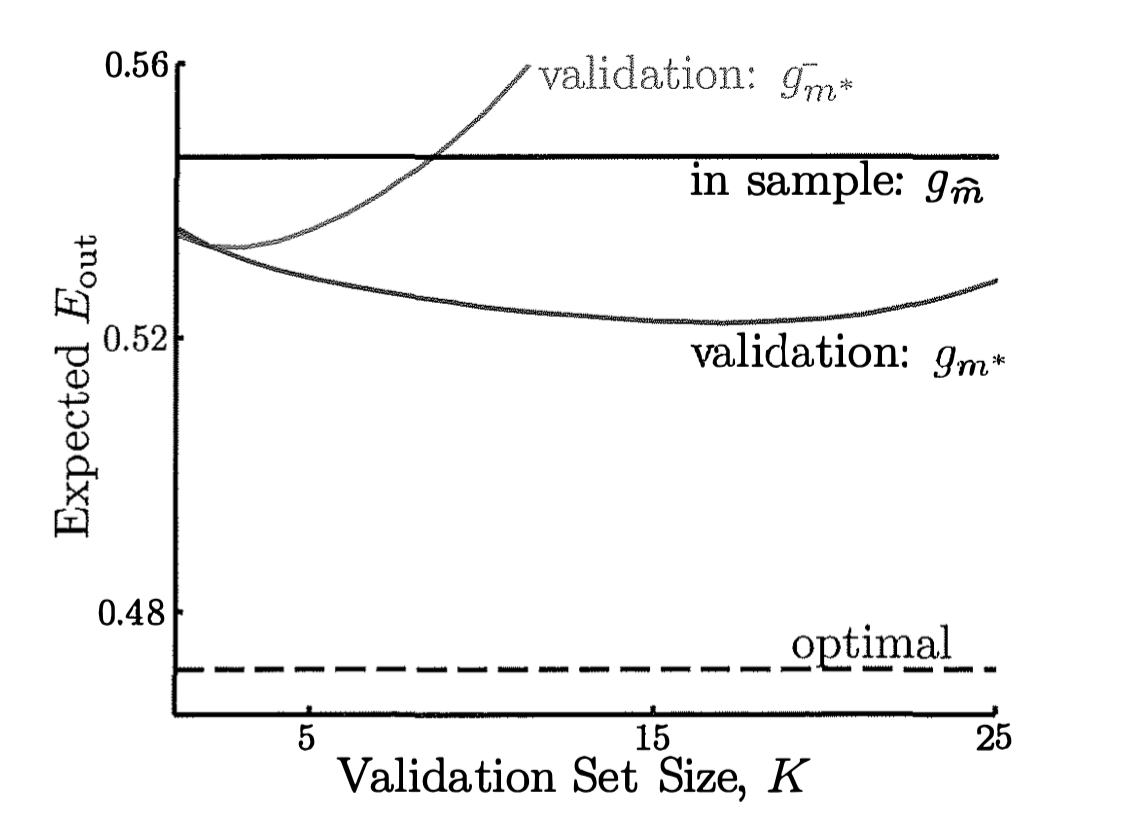
\includegraphics[width=0.7\textwidth]{figure/GeneralizedErrorVsValidationSize.png}
    \caption{Generalized error versus validation set size $K$. \emph{validation $g_{{m}^*}^-$}: the model trained on $\mathcal{D}_{train}$ with the validation set for model selection. \emph{in sample $g_{\hat{m}}$}: the model trained on $\mathcal{D}$ without validation set. \emph{validation $g_{{m}^*}$}: the model that is trained on $\mathcal{D}$ at first for selecting $m^*$ and then is retrained on $\mathcal{D}$ with fixed $m^*$.  
    The dotted line \emph{optimal} is the optimal model selection, if we could select the model based on the true out of sample error.
    }
    \label{fig:problem6fig}
\end{figure}

\begin{thebibliography}{9}
\bibitem{learningfromdata} 
Abu-Mostafa, Yaser S., 1957-. Learning From Data : a Short Course. \emph{[United States] :AMLBook.com}, 2012.


\end{thebibliography}

\end{document} 